\iffalse \bibliography{include/backmatter/magnus,include/backmatter/philip} \fi
\chapter{Data Validation}\label{section:data-validation}

This section introduces the result of executing parts of the experiment on a self-driving Volvo truck, depicted in figure~\ref{truck}, that participated in the Grand Cooperative Driving Challenge (GCDC) 2016 in the Netherlands. \\

\begin{figure}[ht]
\centering
     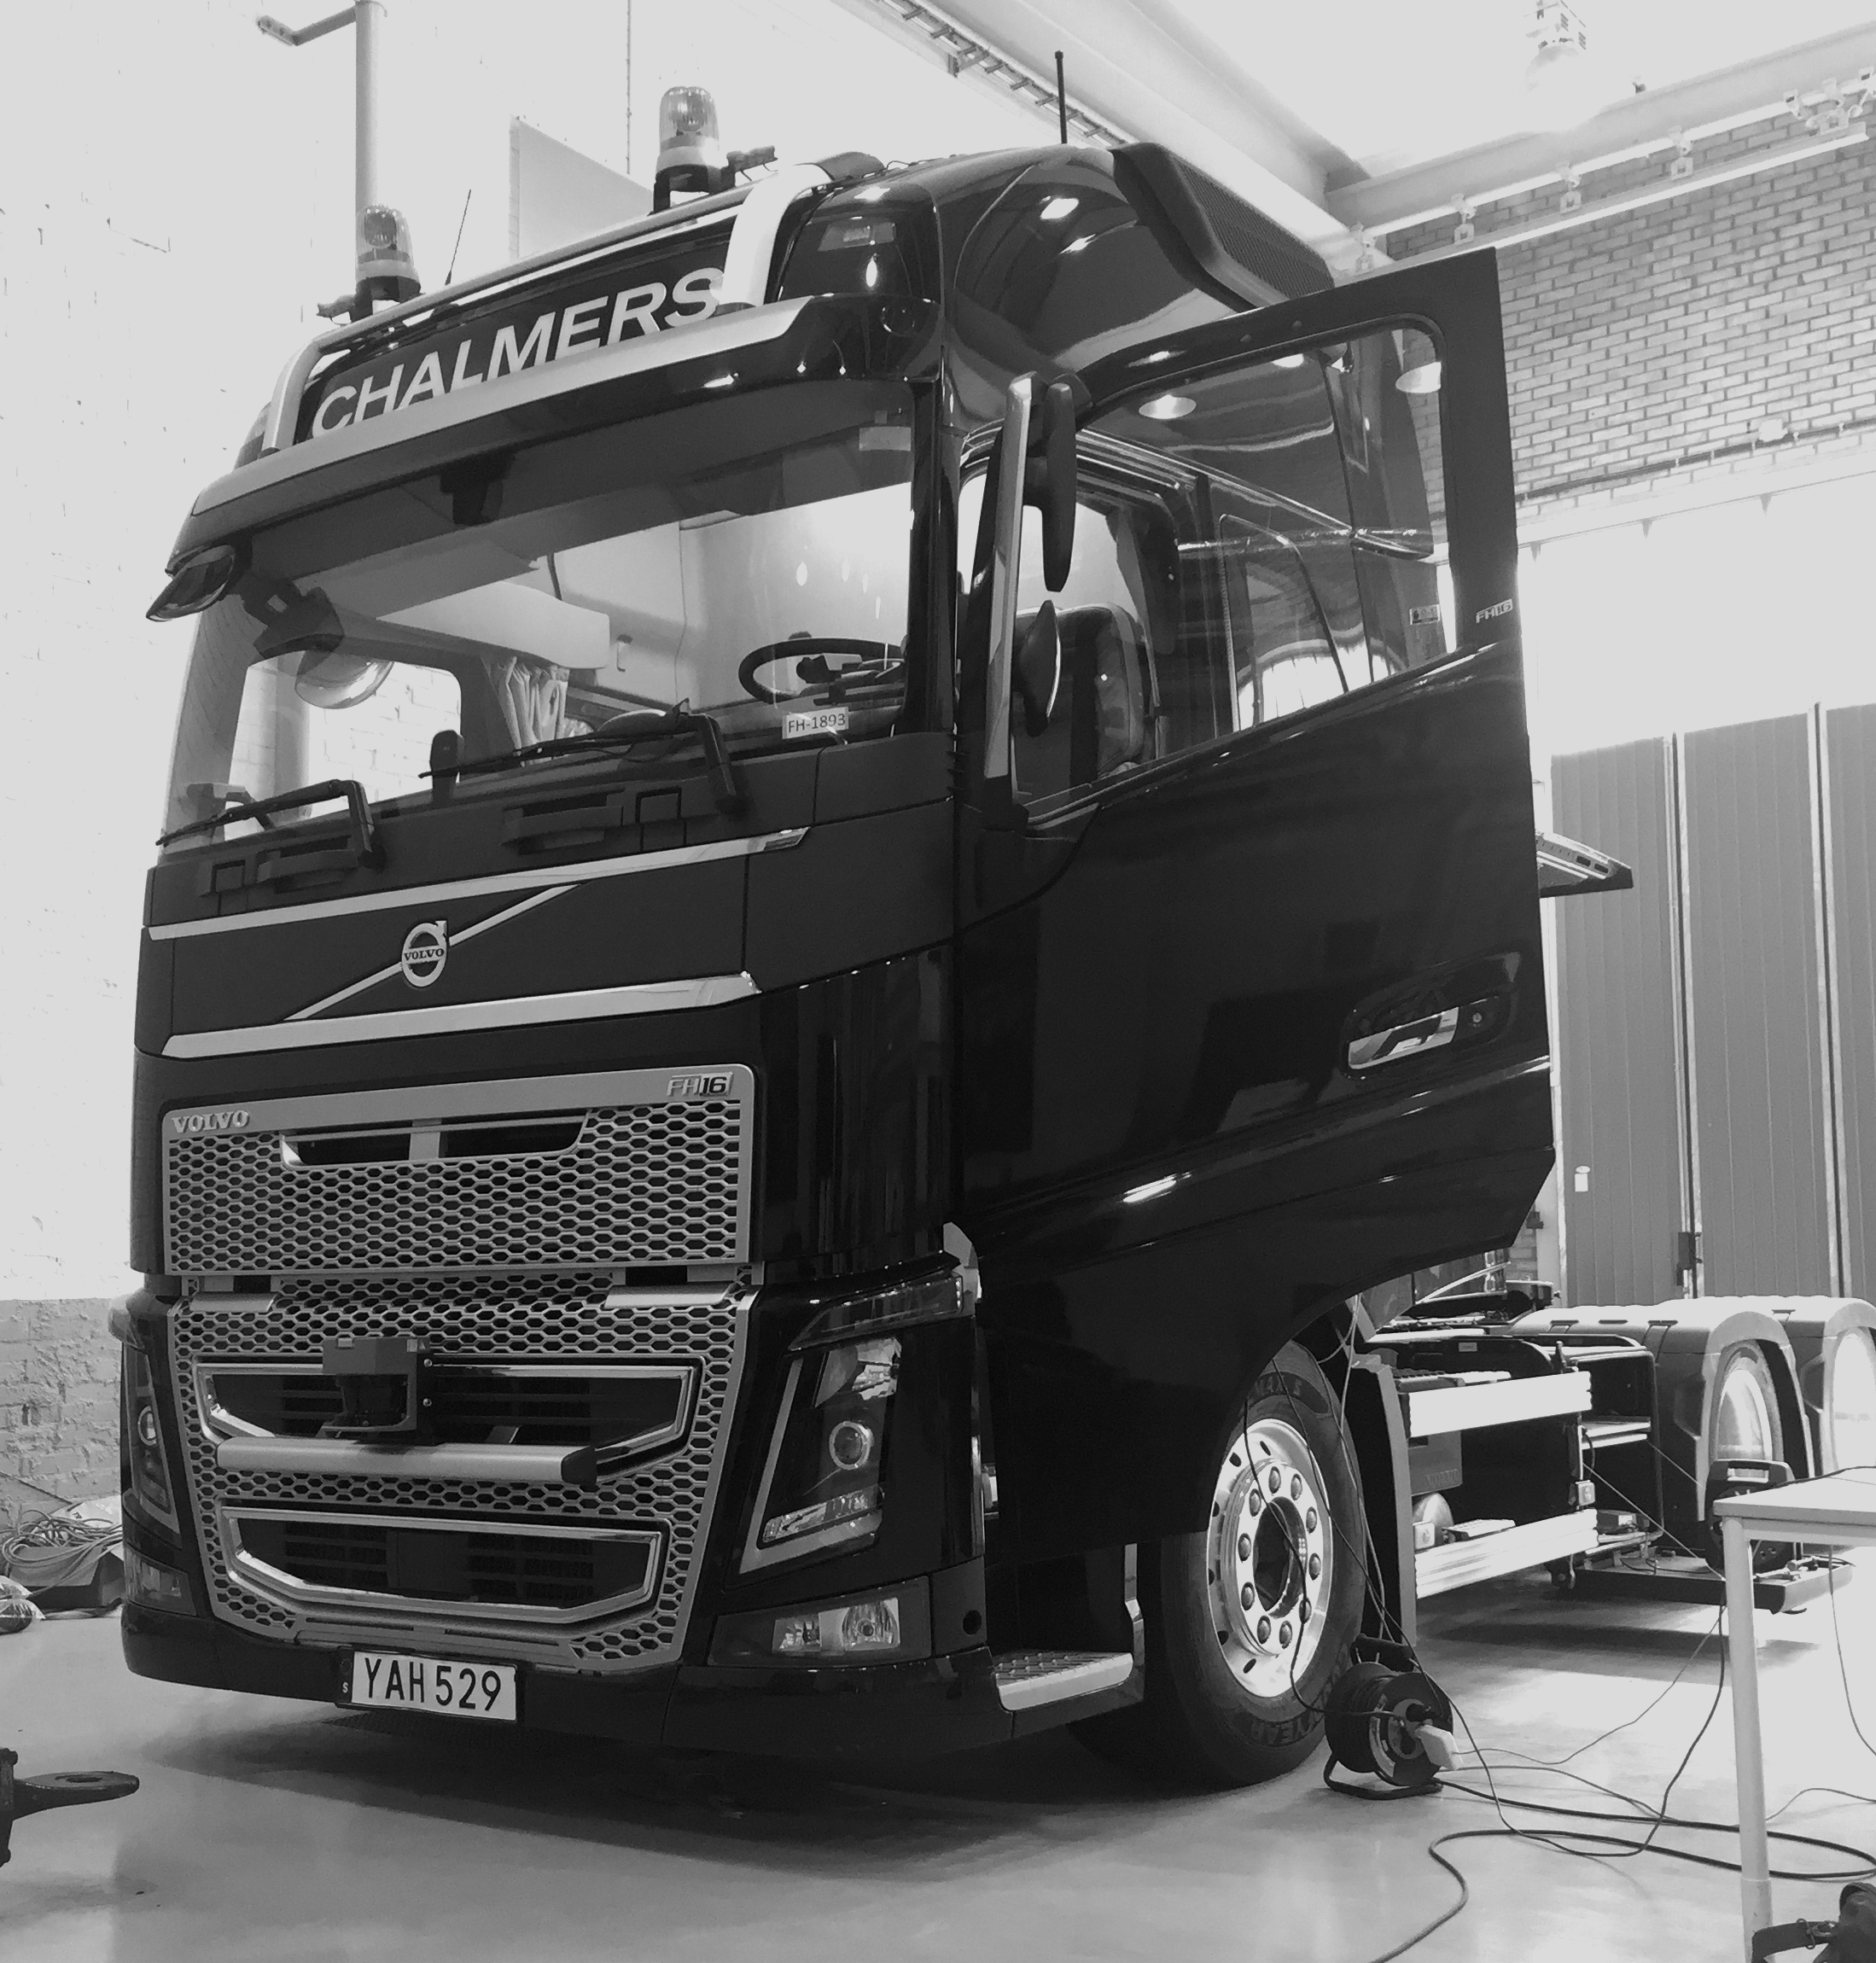
\includegraphics[width=0.4\textwidth]{./figure/truck.png}
      \caption{Chalmers Revere GCDC Truck}
       \label{truck}
\end{figure}


\section{Method}
\label{sec:truck-method}

\subsection{Experimental Units}
\label{sec:truck-expun}

The Pi Component from \ref{section:exp-units} is executed on a target system identical to the one used during the controlled experiments. The computer is connected to hardware components mounted to a Volvo FH16 truck. As the use-case data is extracted using the Pi Component no measurements are done to understand the camera input and disk output performance for the use-case due to the priority of building an understanding of how the scheduling precision behaves with the runtime load of the self-driving truck.\\

To understand how Docker impacts the scheduling precision on the use-case, the experimental unit is executed first natively and secondly within a Dockerised container. The runtime properties of Docker are presented in table \ref{docker-parameters-truck}. Docker version 1.11.1 is used for the analysis procedure and the Docker daemon is set to use the overlayfs storage driver.



\begin{table}[ht]
\begin{tabular}{|l|p{10cm}|}
\hline
\textbf{Parameter}           & \textbf{Description}                                            \\ \hline
\texttt{-d}                  & Run the container in detached mode.                             \\ \hline
\texttt{--net=host}          & The networking configuration is derived from the host.          \\ \hline
\texttt{--cap-add=sys\_nice} & Allow access to devices such as the web camera and the serial port. \\ \hline
\texttt{-v}                  & Mount shared filesystems from the host into the container.    \\ \hline
\texttt{-w}                  & The working directory to execute the experimental units.               \\ \hline
\end{tabular}
\centering
\caption{Docker Image Runtime Properties}
\label{docker-parameters-truck}
\end{table}


\subsection{System Load}
\label{sec:truck-load}

The major difference in comparison to the controlled experiment run is that all software components required for the Volvo truck to operate in a driver-less manner is started and run in the background: this bring a more realistic operational load and consequently a less controlled environment in respect to the controlled experiment. Fifteen components are executed natively and within a Dockerized environment on the target system. These components are tasked with various responsibilities spanning from capturing satellite positioning data, reading data from the vehicle (e.g steering position), vehicle to vehicle communication and a number of camera operating components. Measurement points are captured via serial communication to measure the impact in a real use case.\\

\subsection{Target System}
\label{sec:truck-target}

Table \ref{table:hardware-truck} presents the hardware setup for the target machine upon which the experimental unit (section \ref{sec:truck-expun}) is executed. The target system is running ArchLinux operating system with a real-time enabled kernel (RT\_preempt), version 4.5.0-1.

\begin{table}[ht]
\centering
\begin{tabular}{|l|l|}
\hline
\textbf{Component} & \textbf{Specification}           \\ \hline
Processor          & Intel Core i7 3517UE 1.7 GHz     \\ \hline
Memory             & 4GB DDR3 1333/1600 SODIMM        \\ \hline
Storage Device     & 2.5" SATA HDD x 1                \\ \hline
Serial Interfaces  & \begin{tabular}[c]{@{}l@{}}USB type A x 2 for USB 2.0\\ USB type A x 2 for USB 3.0\\ DB-9 x 2 for RS-232/422/485 x 2\\ DB-9 x 4 for RS-232 x 4 \\ Isolated DB-9 x 2 for RS-232/422/485 x 2
\end{tabular} \\ \hline
\end{tabular}
\caption{Target System Hardware Specification}
\label{table:hardware-truck}
\end{table}



\section{Results}

The results shown in figure \ref{fig:truck-std-chart-noload} show that there exists a difference between the two deployment contexts in the load environment introduced by the other components running on the same system. The difference indicates that the deployment context has an impact on how deterministic a system is as native fluctuates roughly $40\%$ less than the Docker deployment context. Running a statistical test to understand the cause and effect relationship between the deployment context and the dependent variables resulted in a $\eta^{2}=0.504$ which relates to a medium effect size between deployment context and the dependent variables according to Cohen's D ($\eta^{2} > 0.5$). Figure \ref{fig:truck-mean-chart-noload} show that there exists no violations for the average time deadline for either of the two execution environments.


\pgfplotstableread[col sep = semicolon]{data/truck/colsd_load.csv}\mydatanoload
\begin{figure}[ht]
\caption{Standard deviation of execution environments with real-life load \textit{(lower is better)}}
\label{fig:truck-std-chart-noload}
\begin{tikzpicture}
\begin{axis}[
      xbar stacked,
      width=\textwidth*.95,
      height=\textheight*.19,
      xlabel={},
      ytick=data,
      xmin=0,
      % xmax=1.15,
      enlarge y limits={abs=1},
      y dir=reverse,
      xlabel={$ns$ std. dev.},
      yticklabels={Native [RT],Docker [RT]},ytick={1,...,2},
      point meta={x*100},
      legend style={
                draw=none, % ?
                text depth=0pt,
                at={(0.5,-0.38)},
                anchor=north,
                legend columns=-1,
                % default spacing:
                column sep=1cm,
                % the space between legend image and text:
                /tikz/every odd column/.append style={column sep=0cm},
            }
        ] %first axis

\addplot+[draw opacity=0,fill=orange,xbar,area legend] table[y=scenario,x=odv_oh1]{\mydatanoload};
\addplot+[draw opacity=0,fill=blues3,xbar,area legend] table[y=scenario,x=pi_calc]{\mydatanoload};
\addplot+[draw opacity=0,fill=blues5,xbar,area legend] table[y=scenario,x=odv_oh2]{\mydatanoload};
\addplot+[draw opacity=0,fill=blues1,xbar,area legend] table[y=scenario,x=sleep]{\mydatanoload};

\legend{\scriptsize Overhead 1,\scriptsize Pi calculation,\scriptsize Overhead 2,\scriptsize Sleep};
\end{axis}
\end{tikzpicture}
\end{figure}


\pgfplotstableread[col sep = semicolon]{data/truck/colsum_load.csv}\mydatanoload
\begin{figure}[ht]
\caption{Mean consumed of time-slice with use-case load \textit{(closer to 100\% is better)}}
\label{fig:truck-mean-chart-noload}
\begin{tikzpicture}
\begin{axis}[
        xbar stacked,
        width=\textwidth*.95,
        height=\textheight*.19,
        xlabel={},
        ytick=data,
        xmin=0,
        xmax=1.15,
        y dir=reverse,
        xlabel={$\%$ of time-slice},
        enlarge y limits={abs=1},
        yticklabels={Native [RT],Docker [RT]},ytick={1,...,2},
          x label style={at={(axis description cs:0.5,-0.1)},anchor=north},
        xticklabel={\scriptsize\pgfmathparse{\tick*100}\pgfmathprintnumber{\pgfmathresult}\%},
        point meta={x*100},
        legend style={
                draw=none, % ?
                text depth=0pt,
                at={(0.5,-0.35)},
                legend cell align=left,
                anchor=north,
                legend columns=-1,
                % default spacing:
                column sep=1cm,
                % the space between legend image and text:
                /tikz/every odd column/.append style={column sep=0cm},
            }
        ] %first axis


\draw[black, dotted] (axis cs:1,-2) -- (axis cs:1,11);
\addplot+[draw opacity=0,fill=orange,xbar,area legend] table[y=scenario,x=odv_oh1]{\mydatanoload};
\addplot+[draw opacity=0,fill=blues3,xbar,area legend] table[y=scenario,x=pi_calc]{\mydatanoload};
\addplot+[draw opacity=0,fill=blues5,xbar,area legend] table[y=scenario,x=odv_oh2]{\mydatanoload};
\addplot+[draw opacity=0,fill=blues1,xbar,area legend] table[y=scenario,x=sleep]{\mydatanoload};

\legend{\scriptsize Overhead 1,\scriptsize Pi calculation,\scriptsize Overhead 2,\scriptsize Sleep};
\end{axis}
\end{tikzpicture}
\end{figure}
